\documentclass[a4paper]{article}
\usepackage{cmap}
\usepackage[utf8]{inputenc}
\usepackage[T2A]{fontenc}
\usepackage[english,russian]{babel} 
\usepackage[left=15mm, top=15mm, right=15mm, bottom=42mm, nohead, nofoot]{geometry}
\usepackage{graphicx}  % изобржаения
\usepackage{float} % плавающие объекты
\usepackage{wrapfig}  % изобржаения
\usepackage{blindtext} % рыба-текст
\usepackage{tikz} % графика
\usepackage{xcolor} % определение цветов
\usepackage{nicefrac} % красивые дроби
\usepackage{cancel} % сокращение
\usepackage{amsmath,amsfonts,amssymb} % математический пакет
\usepackage{hyperref}  % гиперссылки
\usepackage{fancybox,fancyhdr} % хедер и футер
\pagestyle{fancy}
\fancyhf{}
\fancyhead[L]{РГР №3}
\fancyhead[R]{Дифференциальные уравнения}
\fancyfoot[C]{\thepage}
\setcounter{page}{1}
\headsep=10mm
\footskip=10mm

\addto\captionsrussian{
  \renewcommand{\contentsname}
    {\centering Содержание}
}
\newcommand{\addsection}[1]{\addcontentsline{toc}{section}{#1}
\section*{\centering #1}}
\newcommand{\addsubsection}[1]{\addcontentsline{toc}{subsection}{#1}
\subsection*{\centering #1}}

\newcommand\NB{\textbf{N\kern-0.32em\textcolor{red}{B}}:\quad}

\begin{document}
\begin{titlepage}
    \begin{center}
        Министерство образования и науки Российской Федерации \\
        Федеральное государственное автономное образовательное учреждение \\ высшего образования \\[6pt]
        САНКТ-ПЕТЕРБУРГСКИЙ НАЦИОНАЛЬНЫЙ \\ ИССЛЕДОВАТЕЛЬСКИЙ УНИВЕРСИТЕТ ИТМО \\[25em]
        Практическая работа \\[0.5em]
        \textbf{ЧИСЛЕННЫЕ МЕТОДЫ РЕШЕНИЯ\\УРАВНЕНИЙ ВЫСШИХ ПОРЯДКОВ}
    \end{center}\,\\[8.5em]
    \begin{flushright}
        Студенты: Овчинников П.А.\\
        Румянцев А.А. \\
        Чебаненко Д.А. \\[1em]
        Группа: R3241
    \end{flushright}\,\\[8.5em]
    \begin{center}
        {\small Санкт-Петербург \\ 2023}
    \end{center}
\end{titlepage}
\tableofcontents\,\\[1em]
Численные методы решения дифференциальных уравнений высших порядков --- методы, которые решают дифференциальные уравнения, представляя результат в виде набора чисел. Чаще всего такие методы имеют чёткий алгоритм, поэтому их реализация в компьютерных программах не вызывает трудностей. Иногда для решения задачи требуется применение сразу нескольких численных методов, и вот какие из них существуют:
\begin{enumerate}
    \item Метод Эйлера
    \item Метод Рунге-Кутта
    \item Метод Адамса
    \item Метод стрельбы
    \item Метод конечных разностей
    \item Метод конечных элементов
    \item Метод Галёркина
    \item Метод Ритца
\end{enumerate}
Как следует из содержания, в данной работе мы рассмотрим первый, второй и четвёртый методы.
\addsection{Метод Эйлера}
\addsubsection{В чем заключается суть метода Эйлера?}
Идея метода Эйлера заключается в аппроксимации интегральной кривой кусочно-линейной функцией,
называемой ломаной Эйлера. Чтобы применить численный метод Эйлера к дифференциальному уравнению
высшего порядка, необходимо свести заданное уравнение к системе уравнений первого порядка. В следующих
пунктах преобразования и метод будут подробно рассмотрены.\\[2mm]
За простоту алгоритма мы платим погрешностью полученной ломаной -- она будет достаточно большая,
так как она систематически возрастает на каждом новом шагу -- явный метод Эйлера является одношаговым первого порядка точности.
Для уменьшения погрешности были придуманы модифицироанный метод Эйлера с пересчетом, где добавляется коррекция прогноза,
вследствие чего достигается второй порядок точности, и двухшаговый метод Адамса-Башфорта,
где используются несколько вычисленных ранее значений функции.\\[2mm]
С учетом всех минусов и доступных более практичных методов кажется, что данный метод использовался ранее до появления
более точных аналогов, а сейчас устарел и нигде не применяется, но на самом деле в виду своей простоты данный алгоритм
находит свое применение в теоретических исследованиях дифференциальных уравнений, задач вариационного исчисления и ряда
других математических проблем.

\addsubsection{Теоретическая справка}
Рассмотрим основной принцип метода Эйлера на самом простом примере, еще без уравнений высших порядков.
Пусть дана задача Коши для уравнения первого порядка:
$$\frac{dy}{dx}=f(x,y),\quad y|_{x=x_0}=y_0,$$
где функция $f$ определена на некоторой области $D\subset \mathbb{R}^2$. Решение ищется на полуинтервале $(x_0, b]$.
Разобьем интервал на $n$ равных частей и получим шаг сетки $h=\nicefrac{(b-x_0)}{n},$ иными словами введем на промежутке узлы
$x_0<x_1<\ldots<x_n\leq b$. Приближенное решение в узлах $x_i,$ которое обозначим через $y_i,$ определяется по формуле:
$$y_i=y_{i-1}+(x_i-x_{i-1})f(x_{i-1},y_{i-1})\equiv y_{i-1}+hf(x_{i-1},y_{i-1}),\quad i=1,2,3,\ldots ,n$$
Как уже было написано в предыдущем пункте, метод Эйлера решает только уравнения первого порядка, а значит нам
придется приводить уравнение высшего порядка к системе уравнений первого порядка и решать каждое по отдельности по этому принципу.\\[2mm]
\NB Другими словами метод Эйлера основан на дискретизации дифференциальных уравнений во времени.
\addsubsection{Алгоритм}
Любое дифференциальное уравнение $m$-го порядка $$y^{(m)}=f(x,y,y^{\prime},y^{\prime\prime},\ldots,y^{(m-1)})$$ можно свести
к системе, состоящей из $m$ уравнений первого порядка при помощи замен. Проведем следующие замены:
\vspace{-2.5mm}
\begin{align*}
    & y_1=y^{\prime},\\
    & y_2=y^{\prime\prime}=y_1^{\prime},\\
    & y_3=y^{\prime\prime\prime}=y_2^{\prime},\\
    & \vdots\\
    & y_m=y^{(m)}=y_{m-1}^{\prime}
\end{align*}
В результате дифференциальное уравнение $m$-го порядка сводится к системе, состоящей из $m$ дифференциальных
уравнений первого порядка:
\begin{equation*}
    y^{(m)}(x)=
    \begin{cases}
        y^{\prime}=y_1\\
        y_1^{\prime}=y_2\\
        y_2^{\prime}=y_3\\
        \vdots\\
        y_{m-1}^{\prime}=f(x,y,y_1,y_2,\ldots,y_{m-1})
    \end{cases}
\end{equation*}
Применим метод Эйлера к каждому уравнению в системе, тогда расчетные формулы примут вид:
\begin{equation*}
    y^{(m)}(x)=
    \begin{cases}
        y_{n+1}=y_n+h\cdot y_{1,n}\\
        y_{1,n+1}=y_{1,n}+h\cdot y_{2,n}\\
        y_{2,n+1}=y_{2,n}+h\cdot y_{3,n}\\
        \vdots\\
        y_{m-1,n+1}=y_{m-1,n}+ hf(x_n,y_n,y_{1,n},y_{2,n},\ldots,y_{m-1,n})\\
        x_{n+1}=x_n+h
    \end{cases}
\end{equation*}
\noindent где $y_n,y_{1,n},y_{2,n}\ldots y_{m-1,n}$ -- значения переменных на текущем шагу,
а $y_{n+1},y_{1,n+1},y_{2,n+1}\ldots y_{m-1,n+1}$ -- значения на следующем шагу.\clearpage\noindent
Каждое из уравнений в системе будет являться решением заданного дифференциального уравнения высшего
порядка. Можно построить график зависимости конкретного уравнения из системы от времени $x$ и получить
приблеженное решение соответствующего ДУ высшего порядка.\\[2mm]
Если заданное дифференциальное уравнение высшего порядка является неоднородным $(g(x)\neq 0)$
$$y^{(m)}=f(x,y,y^{\prime},y^{\prime\prime},\ldots,y^{(m-1)})+g(x),$$ то его решением также
будет являться система уравнений первого порядка, а неоднородность
будет учитываться в уравнении самого высокого порядка:
\begin{equation*}
    y^{(m)}(x)=
    \begin{cases}
        y_{n+1}=y_n + h \cdot y_{1,n} \\
        y_{1,n+1}=y_{1,n} + h \cdot y_{2,n} \\
        y_{2,n+1}=y_{2,n} + h \cdot y_{3,n} \\
        \vdots \\
        y_{m-2,n+1}=y_{m-2,n} + h \cdot y_{m-1,n} \\
        y_{m-1,n+1}=y_{m-1,n} + h\left[f(x_n, y_n, y_{1,n}, y_{2,n}, \ldots, y_{m-1,n}) + g(x_n)\right] \\
        x_{n+1}=x_n + h
    \end{cases}
\end{equation*}
\addsubsection{Пример}
Пусть у нас есть линейное неоднородное дифференциальное уравнение третьего порядка
$$y^{\prime\prime\prime}(x)+2y^{\prime\prime}(x)-y^{\prime}(x)+1=e^x$$
с начальными условиями
$$x_0=0,\quad y(x_0)=1,\quad y^{\prime}(x_0)=0,\quad y^{\prime\prime}(x_0)=2.$$
Сделаем следующие замены
$$y_1=y,\quad y_2=y^{\prime},\quad y_3=y^{\prime\prime},$$
тогда имеем такую систему ДУ первого порядка:
\begin{equation*}
    y^{\prime\prime\prime}(x)=
    \begin{cases}
        y_{1,n+1}=y_{1,n} + h \cdot y_{2,n} \\
        y_{2,n+1}=y_{2,n} + h \cdot y_{3,n} \\
        y_{3,n+1}=y_{3,n} + h(-2y_{3,n}+y_{2,n}-1+e^{x_n}) \\
        x_{n+1}=x_n + h
    \end{cases}
\end{equation*}
\noindent Имеем $x_0=0\Rightarrow y_{1,0}=1,\,y_{2,0}=0,\,y_{3,0}=2$.
Рассмотрим работу алгоритма для простоты при малых значениях $b$ и $n$.
Пусть $b=0.5,\,n=2,\,h=0.25$. Имеем следующие системы:
\begin{equation*}
    n=0,\,\,y^{\prime\prime\prime}(x)=
    \begin{cases}
        y_{1,1}=y_{1,0} + h \cdot y_{2,0} \\
        y_{2,1}=y_{2,0} + h \cdot y_{3,0} \\
        y_{3,1}=y_{3,0} + h(-2y_{3,0}+y_{2,0}-1+e^{x_0}) \\
        x_{1}=x_0 + h
    \end{cases}
    \Rightarrow\,\,\,\,\,\,
    \begin{cases}
        y_{1,1}=1 \\
        y_{2,1}=0.5 \\
        y_{3,1}=1 \\
        x_{1}=0.25
    \end{cases}
\end{equation*}
\begin{equation*}
    n=1,\,\,y^{\prime\prime\prime}(x)=
    \begin{cases}
        y_{1,2}=y_{1,1} + h \cdot y_{2,1} \\
        y_{2,2}=y_{2,1} + h \cdot y_{3,1} \\
        y_{3,2}=y_{3,1} + h(-2y_{3,1}+y_{2,1}-1+e^{x_1}) \\
        x_{2}=x_1 + h
    \end{cases}
    \Rightarrow\,\,\,\,\,\,
    \begin{cases}
        y_{1,2}=1.125 \\
        y_{2,2}=0.75 \\
        y_{3,2}=0.696 \\
        x_{2}=0.5
    \end{cases}
\end{equation*}
\begin{equation*}
    n=2,\,\,y^{\prime\prime\prime}(x)=
    \begin{cases}
        y_{1,3}=y_{1,2} + h \cdot y_{2,2} \\
        y_{2,3}=y_{2,2} + h \cdot y_{3,2} \\
        y_{3,3}=y_{3,2} + h(-2y_{3,2}+y_{2,2}-1+e^{x_2}) \\
        x_{3}=x_2 + h
    \end{cases}
    \Rightarrow\,\,\,\,\,\,
    \begin{cases}
        y_{1,3}=1.3125 \\
        y_{2,3}=0.924 \\
        y_{3,3}=0.6975 \\
        x_{3}=0.75
    \end{cases}
\end{equation*}
Мы решили неоднородное линейное ДУ третьего порядка методом Эйлера с заданными начальными
условиями, интервалом, количеством шагов и шагом сетки. Теперь можно построить три графика -- 
$y_{1,n}(x_n),\,y_{2,n}(x_n),\,y_{3,n}(x_n),$ где $n\in[0,2]$, чтобы получить приближенные
графики заданного ДУ.


\addsection{Метод Рунге-Кутта}
Метод Рунге-Кутты является численным методом решения обыкновенных дифференциальных уравнений (ОДУ) и применяется для аппроксимации решений дифференциальных уравнений. Он особенно эффективен для решения систем ОДУ и уравнений высших порядков. Для уравнения высшего порядка метод Рунге-Кутты применяется после его преобразования в систему уравнений первого порядка.\\[2mm]
Любое дифференциальное уравнение $m$-ого порядка:
\[y^{m} = f(x, y, y', ..., y^{m-1})\]
можно свети к системе, состоящей из m уравнений первого порядка при помощи замен.
\[y_1 = y'\]
\[y_2=y''=y_1'\]
\[y_3=y'''=y_2'\]
\[...\]
\[y_m=y^{(m)} = y^{(m-1)}\]
В результате дифференциальное уравнение $m$-го порядка сводится к системе, состоящей из $m$ дифференциальных уравнений первого порядка:
\begin{align*}
    \begin{cases}
        y' = y_1\\
        y'_1 = y_2\\
        y_2'=y_3\\
        ...\\
        y'_{m_1} = f(x, y, y_1, y_2, ..., y_{m_1})
    \end{cases}
\end{align*}
Решением системы, а значит и дифференциального уравнения m-ого порядка является m табличных функций 
\[y, y_1 = y' \cdot y_2  = y''_2 = y_{m-1}\]
то есть функция $y_x$ и все ее производные включая производную $(m-1)$-го порядка. При этом каждая итз табличных функция определяется на промежутке [a, b] с шагом h и включает n узловых точек. Таким образом, численным решением уравнения или системы является матрица порядка $m \times n$.\\
Дальше применяется метод Рунге-Кутты для уравнений первого порядка.

\addsubsection{Пример}
Пусть надо решить дифференциальное уравнение
\[y''-xy'+2xy=0.8\] 
с краевыми условиями \[y(1.5) = -0.2\]
\[y'(1.5) = 2\]
Заданные параметры:
\begin{enumerate}
    \item диапазон изменения аргумента [1.5; 2.5]
    \item шаг изменения аргумента h = 0.1
    \item решение --- значения у при x = 1.5; 1.6; ...; 2.5
\end{enumerate}
\clearpage\noindent Заменяем уравнение второго порядка на систему уравнений первого порядка, введя функцию $z(x) = y'(x)$ и выразив производные:
\[z' = U(x, y, z) = xz - 2xy + 0.8\]
\[y' = V(x, y ,z) = z\]
при краевых условиях\\
\[y(1.5) = -0.2\]
\[z(1.5) = 2\]
В методе Рунге-Кутта значение функции в узле ищут по значению функции в предыдущем узле.
\[z_{i+1} = z_i + \frac{h}{6}(q_0+2q_1+2q_2+q_3)\]
\[y_{i+1} = y_i + \frac{h}{6}(k_0 + 2k_1 + 2k_2 + k_3)\] где
\[q_0 = U(x_i, y_i, z_i)\]
\[q_1 = U(x_i + \frac{h}{2}, y_i + k_0\frac{h}{2}, z_i + q_0 \frac{h}{2})\]
\[q_2 = U(x_i + \frac{h}{2}), y_i + k_1 \frac{h}{2}, z_i+q_1\frac{h}{2}\]
\[q_3 = U(x_i + h, y_i + k_2h, z_i + q_2h)\]
\[k_0 = V(z_i)\]
\[k_1 = V(z_i + q_0\frac{h}{2})\]
\[k_2 = V(z_i + q_1\frac{h}{2})\]
\[k_3 = V(z_i + q_2h)\]
Решим задачу Коши методом Рунге-Кутта четвертого порядка, разделив интервал на 10 частей.
\begin{figure}[H]
    \centering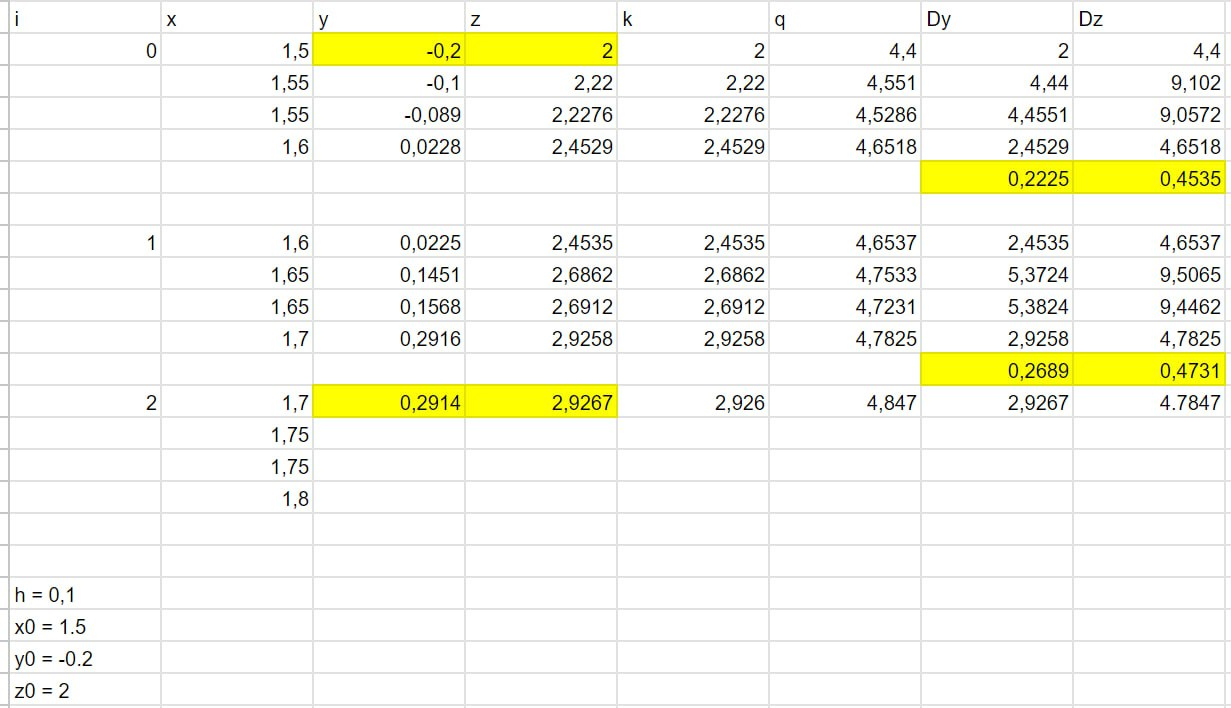
\includegraphics[width=0.7\textwidth]{rk-method.jpg}
\end{figure}


\addsection{Метод стрельбы}
\textbf{Метод стрельбы} --- численный метод решения краевой задачи для дифференциальных уравнений любого порядка. Краевые задачи являются задачами, в которых необходимы найти решение, удовлетворяющее заданным границам. Рассмотрим уравнение второго порядка (\textit{для уравнений более высоких порядков метод стрельбы применяется аналогично, а уравнение n-го порядка сводится к системе из n дифференциальных уравнений первого порядка}):
$$y''(x) = f(x, y, y')$$
Здесь $y(x)$ --- искомая функция, $f(x, y, y')$ --- заданная функция. Также заданы граничные условия ниже:
$$\begin{aligned}
    y(0) &= a \\
    y(l) &= b
\end{aligned}\qquad 0 < x < l$$
Преобразуем уравнение, приведя его к системе:
$$\begin{cases}
    y' = u \\ u' = f(x, y, u)
\end{cases}$$
Для разрешимости получившейся системы в рамках задачи Коши к условию $y(0)$ необходимо условие $y'(0) = u(0)$. Нам известно, что $y(0) = a$, а вот значение $u(0)$ мы будем подбирать. Зададим экспериментальным путём произвольное значение $u(0) = \lambda_1$ и решим задачу численно любым известным методом (например, методом Рунге-Кутта). Так в координате $x=l$ будет вычислено значение $y(l) = y_1$ --- очевидно, $y_1 \ne b$, поэтому мы решим задачу для другого произвольного значения $u(0) = \lambda_2$ и выясним, ближе или дальше от $b$ находится $y_2$, чем $y_1$. Повторяя этот процесс многократно, применяя разные методы коррекции начального значения (например, метод бисекции), мы найдём такое значение $u(0) = \lambda_n$, что $y_n$ будет находиться достаточно близко к $b$. Таким образом, мы найдём решение, удовлетворяющее граничным условиям.\\[2mm]
Такая коррекция $\lambda$ под начальные условия называется методом стрельбы --- название связано с тем, что путём «недолётов-перелётов» мы определяем подходящее значение $y$, из которого вытекает решение $y(x)$.\\[2mm]
\NB Важно отметить, что метод стрельбы \underline{не гарантирует} нахождения решения, а \underline{лишь приближает} к нему --- необходимая точность решения задаётся условием задачи или экспериментально. К тому же этот метод требует нескольких итераций, поэтому его выбор должен быть обоснованным.
\addsubsection{Пример}
Рассмотрим пример дифференциального уравнения второго порядка и решим его методом стрельбы. Пусть дано уравнение:
$$y''(x)+2y'(x)+y(x) = 0$$
Для него задано начальные условия:
$$\begin{aligned}
    y(0) &= 0 \\ y'(0) &= 1
\end{aligned}$$
Преобразуем это уравнение в систему двух уравнений первого порядка, введя новую переменную $u(x) = y'(x)$:
$$\begin{cases}
    y' = u \\ u' = -2u - y
\end{cases}$$
\clearpage\noindent Теперь мы будем решать эту систему методом стрельбы. Выберем произвольное значение $u(0) = \lambda_1 = 1$. Используем метод Рунге-Кутта для интегрирования системы уравнений ($h$ --- шаг интегрирования, о котором в рамках метода стрельбы будет сказано позже):
$$\begin{aligned}
    k_{1y} &= u \\
    k_{1u} &= -2u - y \\
    k_{2y} &= u + \frac{h}{2}k_{1u} \\
    k_{2u} &= -2\left( u + \frac{h}{2}k_{1u} \right) - \left( y + \frac{h}{2}k_{1y} \right) \\
    k_{3y} &= u + \frac{h}{2}k_{2u} \\
    k_{3u} &= -2\left( u + \frac{h}{2}k_{2u} \right) - \left( y + \frac{h}{2}k_{2y} \right) \\
    k_{4y} &= u + hk_{3u} \\
    k_{4u} &= -2\left( u + hk_{3u} \right) - \left( y + hk_{3y} \right)
\end{aligned}$$
Обновим значения $y$ и $u$ с использованием метода Рунге-Кутта ($y_0 = y(0)$ и $u_0 = y'(0)$ на первой итерации):
$$\begin{aligned}
    y_1 &= y_0 + \frac{h}{6}\left( k_{1y} + 2k_{2y} + 2k_{3y} + k_{4y} \right) \\
    u_1 &= u_0 + \frac{h}{6}\left( k_{1u} + 2k_{2u} + 2k_{3u} + k_{4u} \right)
\end{aligned}$$
Проверяем, насколько близко полученное значение $y_1$ к желаемому $y(0)$. Если они близки для заданной точности, то мы нашли решение. Если нет, то мы повторяем процесс, скорректировав $\lambda_1$  при помощи корректировочной формулы $\lambda_2 = \lambda_1 - \frac{y_1 - y_0}{u_1}$ и повторяем процесс. В общем виде корректировочная формула выглядит так:
$$\lambda_{n+1} = \lambda{n} - \frac{y_n - y_0}{u_n}$$
Остаётся лишь повторять процесс с новым и новым $\lambda$ до тех пор, пока не достигнем достаточной близости.\\[2mm]
\NB Шаг интегрирования $h$ необходимо выбирать внимательно. Решение будет приблежённым, и его точность напрямую зависит от шага интегрирования --- чем меньше шаг, тем точнее решение. Однако слишком маленький шаг может привести к тому, что метод стрельбы не сойдётся к решению. Или же можно использовать более точные методы интегрирования.

\end{document}